\problemname{}
As every Saturday, Eve is paying her local game club a visit.
Today, Bob has brought a new game he has designed on his own.
After thorough investigation, you claim that there exists a dominant strategy, so one player can always win.
Bob is hesitant to accept that his game is boring to play, so he challenges you to play a round!
Since you claim that there exists a dominant strategy, you may determine who begins the game.

\begin{figure}[!h]
  \centering
  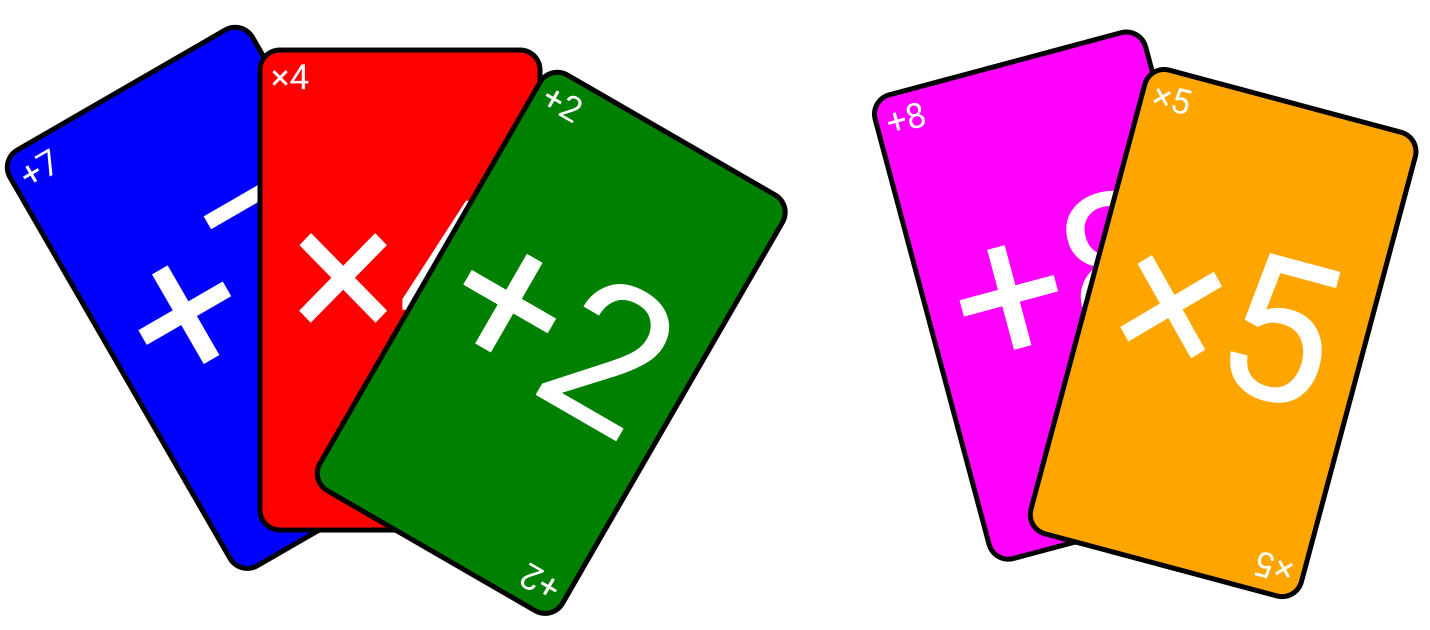
\includegraphics[width=0.78\textwidth]{cards}
  \caption{The cards in the two sample interactions.}
  \label{fig:cards}
\end{figure}

The rules are as follows.
% Consider the following two-player game.
There are $n$ cards on the table, each containing a maths operation (\texttt{+}~or~\texttt{*}) and an integer, as shown in Figure~\ref{fig:cards}.
Eve and Bob alternate picking cards to manipulate a common number using one of the cards.
For instance, if the current value of the number is $5$, and the card says $+3$, then the value gets updated to $8$.
Each card can only be used once, and the game ends when all the cards have been used.
The player who makes the first move wins if the final number is odd, and the other player wins if the final number is even.
%Eve gets to decide who goes first.
Given the list of cards and the starting value, help Eve win the game.

\begin{Interaction}
  The interactor begins by outputting the starting state of the game in the following format:
  \begin{itemize}
    \item One line with an integer $n$ ($1 \le n \le 300$), the number of cards.
    \item $n$ lines, each with a character $o$ and an integer $x$ ($o \in \{$`\texttt{+}'$, $`\texttt{*}'$\}$, $1 \le x \le 10^6$) indicating one of the cards.
    \item One line with an integer $x$ ($1 \le x \le 10^6$), the starting value.
  \end{itemize}
  It is guaranteed that the $n$ cards in the input are distinct.

  Then, your submission must output one of ``\texttt{me}'' or ``\texttt{you}'', depending on if you want to go first or you want the interactor to go first.

  Then your submission and the interactor alternate outputting cards in the same format as above.
  No card can be played more than once.
  Your submission must exit when all cards have been played, regardless of which player made the last move.

  Your submission will be accepted if it follows all the rules above and the final value has the parity indicated on the first line of your output.

  Make sure you flush the buffer after each write.

  A testing tool is provided to help you develop your solution.
\end{Interaction}
